\section{Arquiteturas}

Esse capítulo apresenta diversas arquiteturas possíveis através do 
protocolo OpenFlow. 
O protocolo foi desenvolvido de uma maneira bem aberta para que pudesse 
compreender diversas topologias de rede. 

\subsection{Topologia simples}

Uma topologia simples pode ser vista na figura \ref{fig:simple-topology} onde
um controlador manipula o plano de dados através de um switch OpenFlow 
que possui 3 computadores (\emph{hosts}).

\begin{figure}[h!]
    \centering
    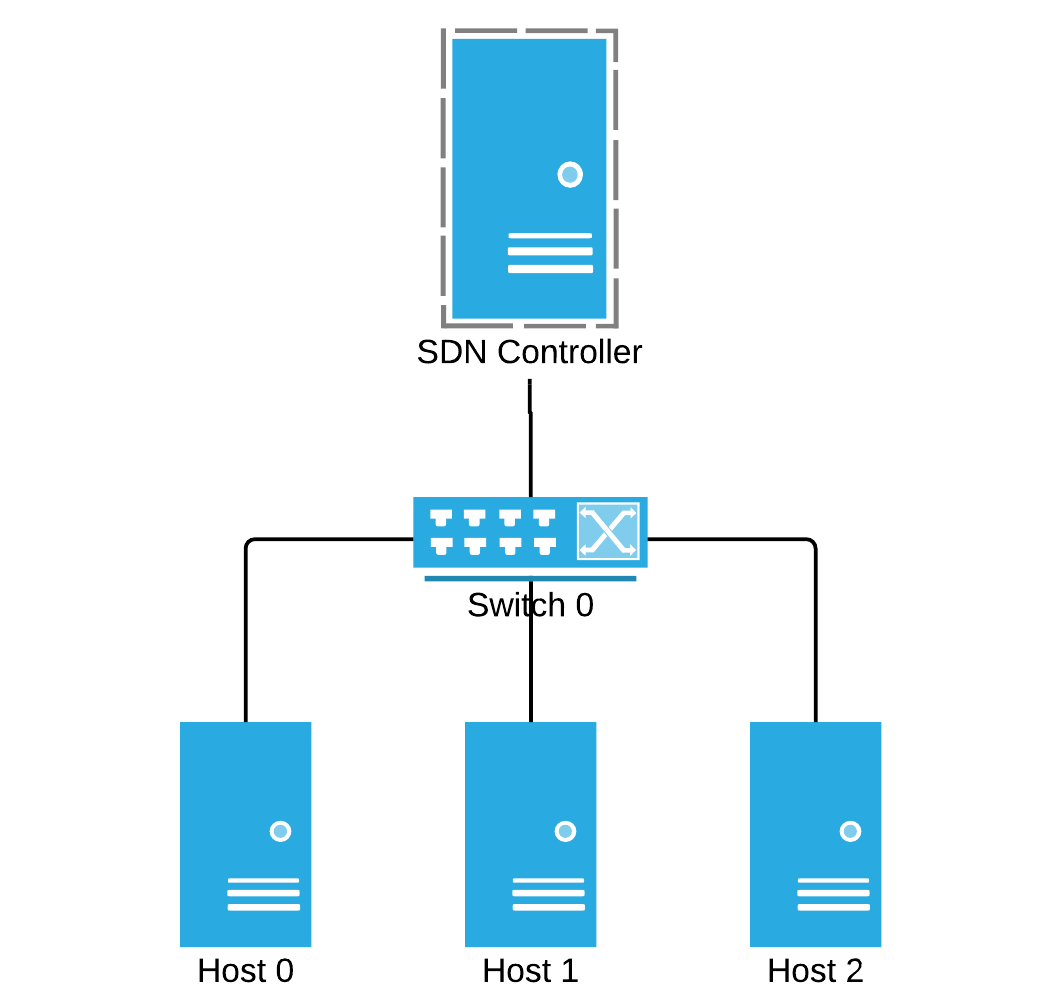
\includegraphics[scale=0.85]{img/simple-topology}
    \label{fig:simple-topology}
    \caption{Topologia simples de redes de computadores}
\end{figure}

Nesse cenário, até mesmo resolução ARP (Address Resolution Protocol) ficam
a cargo do controlador. 
A tabela ARP não é resolvida no switch, mesmo todos as máquinas (hosts) 
estando na mesmo sub-rede. 
Todo as decisões são feitas no plano de controle, logo o controlador 
é quem manipula e atualiza a tabela de fluxos com as regras para 
implementar a resolução de pacotes ARP.

\subsection{Um controlador para \emph{n} switches}

O mesmo controlador pode gerenciar vários switches OpenFlow.
Essa abordagem permite que o controlador tenha uma visão global da topologia
da rede.
Ele pode coletar informações estatísticas e ter controle sobre o estado 
da rede em tempo real.
A figura \ref{fig:controller-n-switches} apresenta essa topologia.

\begin{figure}[h!]
    \centering
    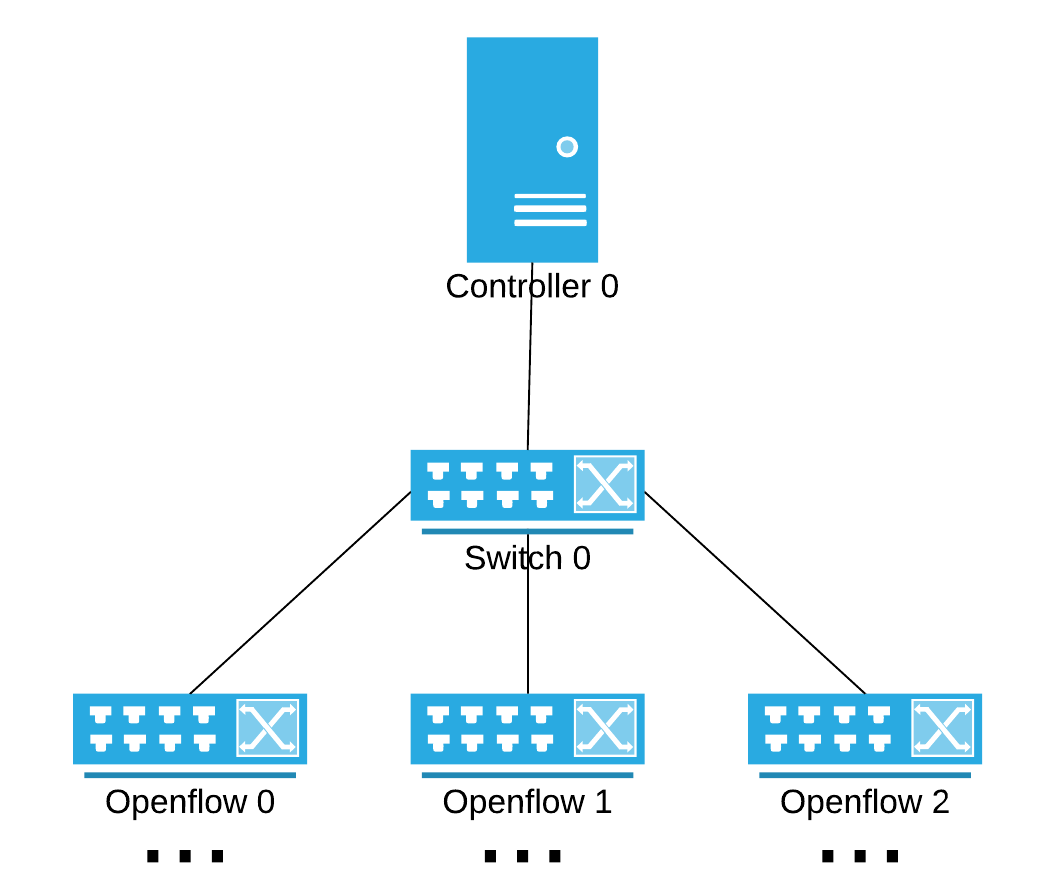
\includegraphics[scale=0.85]{img/controller-n-switches}
    \label{fig:controller-n-switches}
    \caption{Topologia com um controlador e \emph{n} switches}
\end{figure}

É importante notar que os switches podem estar conectados uns aos outros.
A figura \ref{fig:controller-n-linked-switches} mostra um exemplo em que 
dois switches OpenFlow estão conectados entre si.

\begin{figure}[h!]
    \centering
    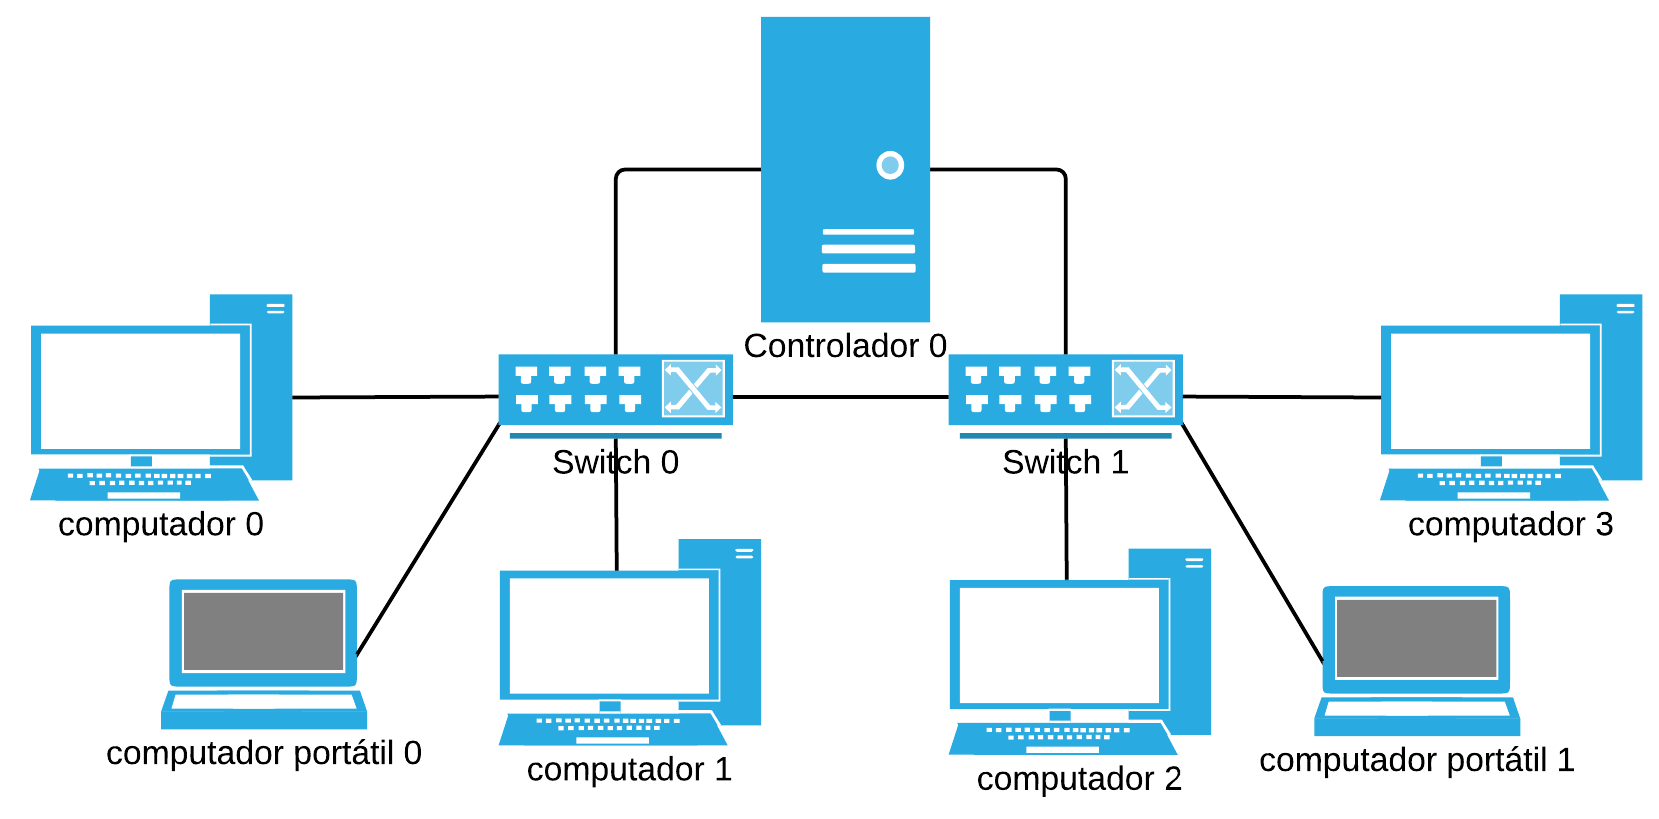
\includegraphics[scale=0.8]{img/controller-n-linked-switches}
    \label{fig:controller-n-linked-switches}
    \caption{Topologia em que os switches OpenFlow 
    estão diretamente conectados}
\end{figure}


\subsection{\emph{n} Controladores para \emph{n} switches}

Diversas sub-redes podem ter seus próprios controladores.
Essa topologia configura um cenário em que não há visão global da rede 
por apenas um controlador. 
Para que esse controle global existisse seria necessário que esses 
controladores trocassem mensagens sobre a topologia da rede.
A figura \ref{fig:n-controllers-n-switches} apresenta um exemplo dessa 
topologia.

\begin{figure}[h!]
    \centering
    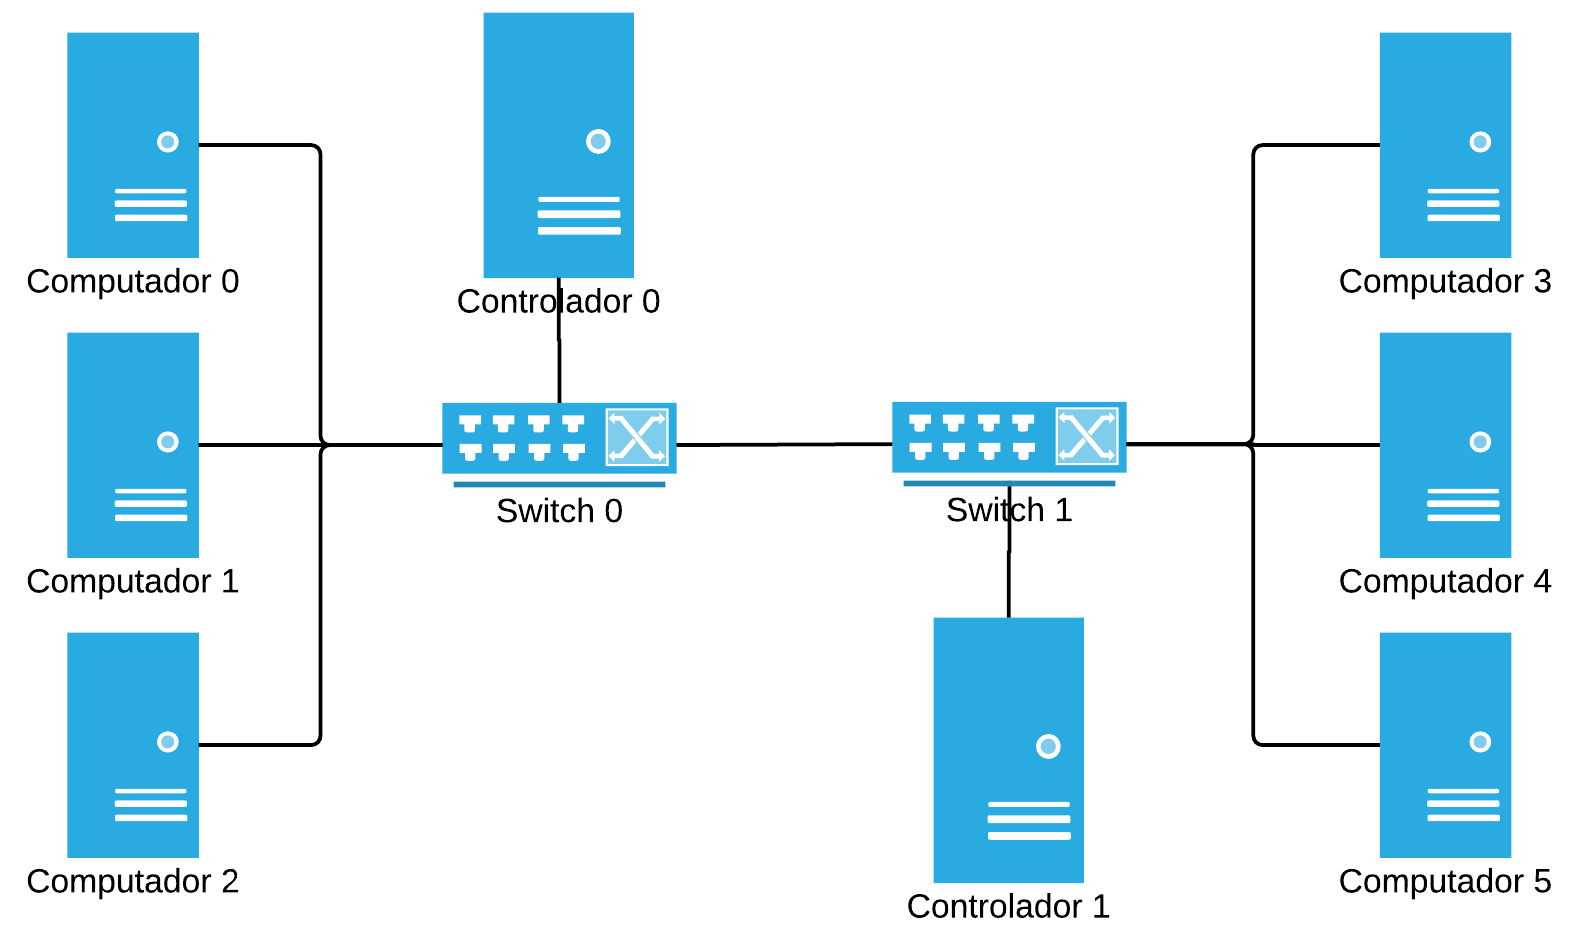
\includegraphics[scale=0.9]{img/n-controllers-n-switches}
    \label{fig:n-controllers-n-switches}
    \caption{Topologia com \emph{n} controladores e \emph{n} switches}
\end{figure}


\subsection{Controlador distribuído}

Um dos fatores mais importantes do protocolo OpenFlow foi permitir que 
uma arquitetura distrubuída pudesse ser aplicada ao controlador da rede.
Sem essa possibilidade, o controlador se torna um gargalo na rede, 
pois à medida que o número de pacotes aumenta, o volume de trabalho do 
controlador cresce. 
Através de uma arquitetura distribuída, o controlador pode dividir a carga 
de trabalho com outros controladores.
É importante ressaltar que mesmo distribuído, a entidade controlador
é tratada como logicamente centralizada.

\begin{figure}[h!]
    \centering
    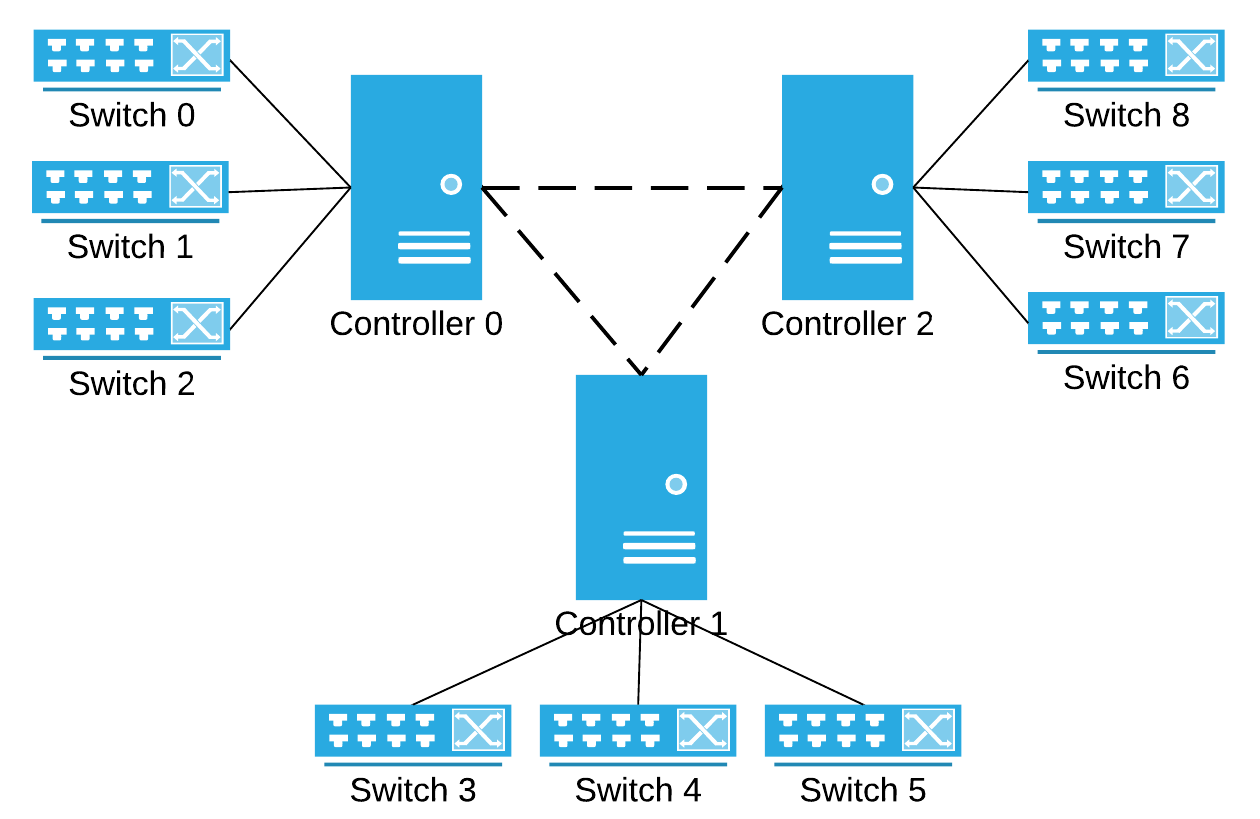
\includegraphics{img/distributed-controller}
    \label{fig:distributed-controller}
    \caption{Topologia de um controlador distribuído}
\end{figure}

Conforme apresentado na figura \ref{fig:distributed-controller}, em uma
arquitetura distribuída, os diversos servidores que compõem o controlador
devem estabelecer um canal de camunicação para que possam trocar mensagens
e tomar decisões de controle da rede de maneira global baseando-se nas
informações contidas em cada um dos servidores.

O protocolo OpenFlow, a partir de sua versão 1.3 permite que o switch seja 
configurado para trabalhar com controladores distribuídos.
Quando operam no modo réplica, os controladores recebem as mesmas mensagens
encaminhadas pelo switch.
Distribuir o controlador torna a rede mais confiável, dado que se um 
controlador cair o switches continuam operando em modo OpenFlow.

Explicar figura e explicar modelo cliente servidor, master e slave, etc do 
OpenFlow.


\subsection{Arquitetura para a Internet}
